\documentclass{ltjsarticle}
\usepackage{amsmath}
\usepackage{amssymb}
\usepackage{ascmac}
\usepackage[dvipdfmx]{graphicx}
\usepackage{tabularx}
\usepackage[colorlinks=true, allcolors=blue]{hyperref}
\usepackage{fancybox}
\usepackage{tikz}
\usepackage{subcaption}
\usetikzlibrary{shapes,arrows}

\begin{document}

\title{101. 深層学習の適用方法(画像認識)}
\author{秋葉洋哉}
\maketitle

\section{ResNet(転移学習)}
\subsection{概要}
学習用のデータが少ない場合に、ImageNetと呼ばれるデータセットを用いて作成された汎用的な画像識別モデルをベースとして、そのモデルに特定のドメインに特化したデータを与えて、学習を行わせることで、簡潔に精度の高い画像識別モデルを作成することができる。この手法を転移学習と呼ぶ。
\par
画像の識別モデルの事前学習として用いられるImageNetは1400万枚以上の画像が収録されており、1000クラス以上のカテゴリに分類されている。ImageNetには、犬や猫、車、飛行機などの画像が収録されており、汎用的な画像識別モデルでは、それらの画像を識別することができる。ImageNetで学習したモデルでは、ResNet50,101,152といったモデルが存在する。

\begin{itembox}{ドメインシフト}
  訓練データとテストデータの分布が異なってしまい、学習したモデルがうまく予測できない現象をドメインシフトと呼ぶ。ドメインシフトの原因は大きく分けて4つに分類できる。
  \begin{enumerate}
    \item 時間的変動 (夏にソフトクリームが良く売れるなど時間によって予測と異なる)
    \item 地域的変動 (大阪でたこ焼きが多く売れるなど地域差によって予測と異なる)
    \item 機器的変動 (搭載機器の性能によって予測と異なる)
    \item 操作的変動 (人それぞれの操作方法や習慣によって予測と異なる)
  \end{enumerate}
  これらのドメインシフトを解消するためには
  \begin{enumerate}
    \item データの再収集
    \item データの拡張 (画像を回転、反転、色調変更)
    \item 転移学習 (大量のデータで訓練された学習したモデルを新しいタスクに転移)
    \item ドメイン適応 (訓練データとテストデータのドメインの違いを数値にしてモデルを学習)
    \item 不変表現学習 (異なるドメインのデータでも共通の特徴表現を学習)
  \end{enumerate}
  といった対策が考えられる。ドメインシフトは実際のビジネスでの機械学習の適用において重要な問題であるため、適切な対策を講じることが求められる。
\end{itembox}

\subsection{ResNet}
ResNetは、2015年にかつてのMicrosoft Researchに所属していたKaiming Heが考案したモデルであり、ImageNetでの画像識別コンペティションで優勝したモデルである(図\ref{fig:Skip_Connection}) 。ResNetは、畳み込み層を152層も積み重ねたモデルであり、SkipConnectionという仕組みを導入し、「元の入力」と「Residual Blockの出力」の二つを「Identity Mapping」と呼ばれる組み合わせ手法で結合することで、層が深くなるにつれて発生する勾配消失問題を回避している(図\ref{fig:Skip_Connection_BackProp})。

\begin{figure}[htbp]
  \centering
  \begin{subfigure}[b]{0.45\textwidth}
    \centering
    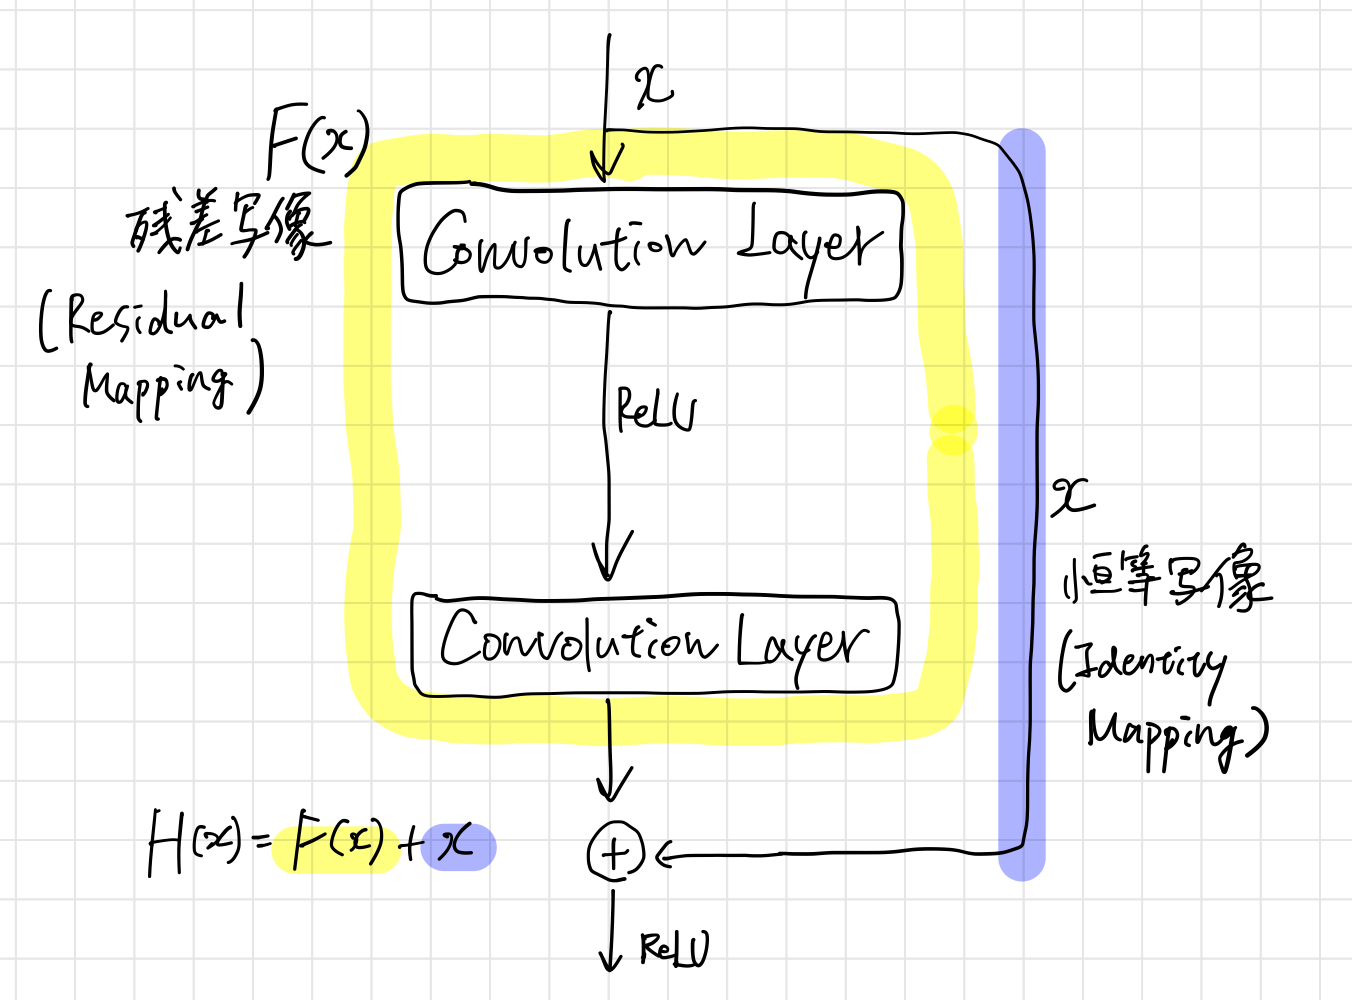
\includegraphics[width=0.8\linewidth]{./capture/Skip_Connection.png}
    \caption{仕組み:学習部分は$F(x)$の残差部分、残差部分のブロックをResidualBlockと呼ぶ。}
    \label{fig:Skip_Connection}
  \end{subfigure}
  \hfill
  \begin{subfigure}[b]{0.45\textwidth}
    \centering
    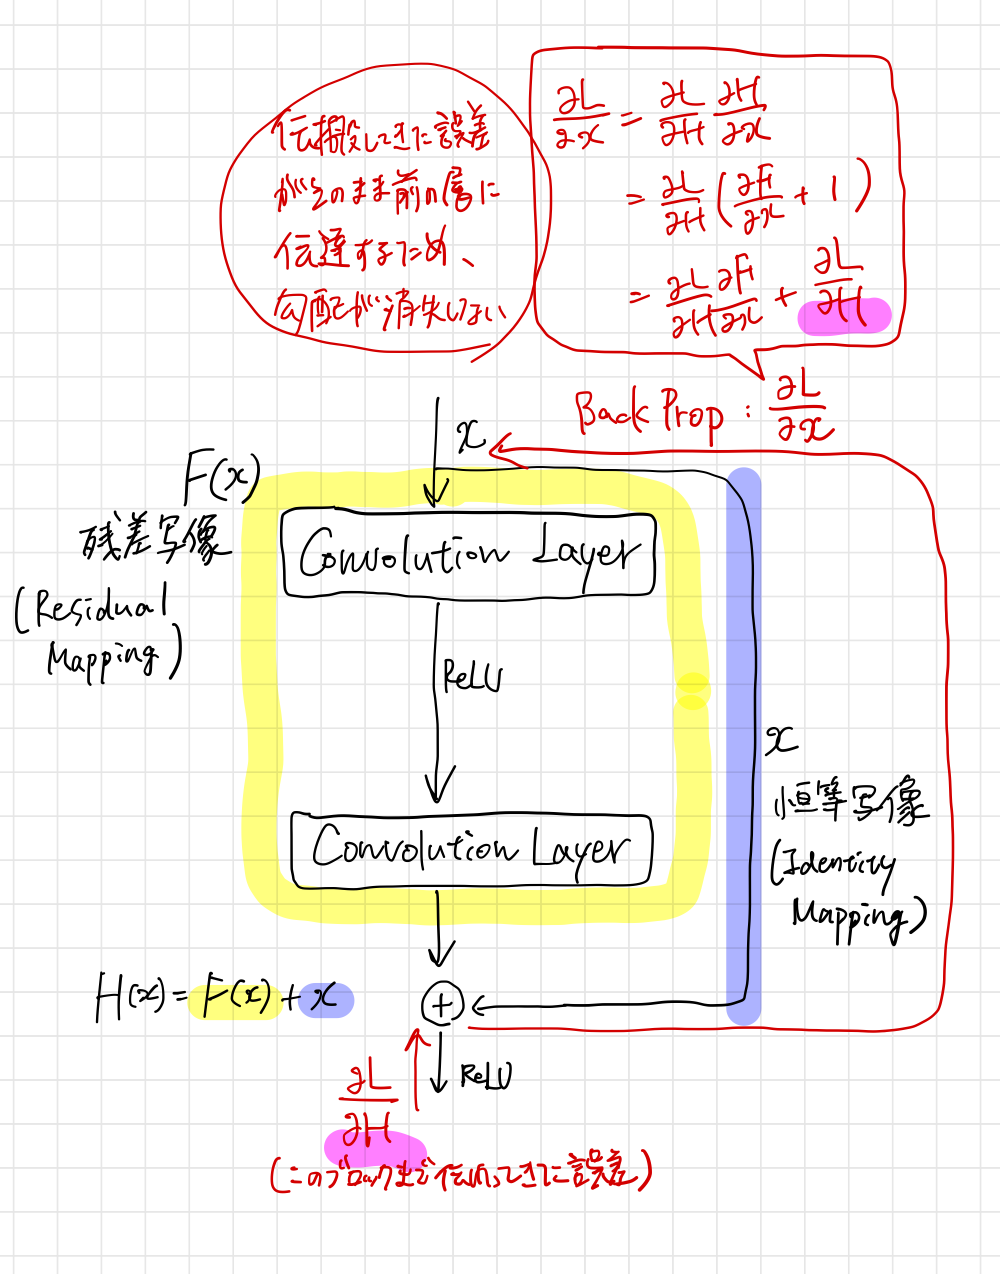
\includegraphics[width=0.8\linewidth]{./capture/Skip_Connection_BackProp.png}
    \caption{勾配消失問題が回避できる理由 : $F(x)$の勾配が消失しても、$x$の勾配が残るため、勾配消失問題を回避できる。}
    \label{fig:Skip_Connection_BackProp}
  \end{subfigure}
  \caption{Skip Connectionについて}
\end{figure}
\par
しかし、ResNetでは、いくつかのブロックだけが有用な表現を学習し、他のブロックは学習が進まないという問題があった。これは、Identity Mappingには、誤差逆伝播時に勾配がResidual Blockを強制的に経由させる仕組みが無いため、何も学習せずスキップしてしまうということが起こるためである。
\par
この問題に対して、層を増やしてパラメータを少なくするために、できるだけ1層あたりの内部構造を薄くしようとした結果、BottleNeckアーキテクチャという仕組みが導入された。BottleNeckアーキテクチャ(図\ref{fig:BottleNeck})は、畳み込み層の前後に1x1の畳み込み層を挟むことで、計算量を削減している。

\begin{figure}[htbp]
  \centering
  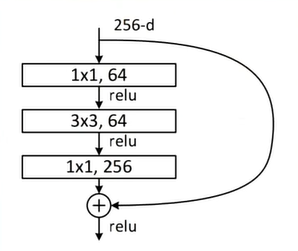
\includegraphics[width=8cm]{./capture/Bottleneck.png}
  \caption{BottleNeckアーキテクチャの仕組み}
  \label{fig:BottleNeck}
\end{figure}
\par
また、無意味な層を減らすという目的のため、Residual Block内の畳み込み層のチャネル方向を広げる、という方針で、WideResNetというモデルが考案された。

\subsection{WideResNet}
ResNetを工夫した、WideResNetは、ResNetの畳み込み層の層数を減らし、フィルタ数を$k$倍に増やしてGPUの特性に合わせることで、高速かつ高精度の学習を可能にしたモデルである。また、残差ブロック内にDropoutを導入することで、過学習を抑制している。
\par
まず、Residual Blockの表現力を向上させる方法は、以下の3つが考えられる。
\begin{enumerate}
  \item ブロックにより多くの畳み込み層を加える
  \item より多くの特徴平面を加えることで畳み込み層を広げる
  \item 畳み込み層のフィルタサイズを大きくする
\end{enumerate}
このうち、1, 2を実現しようとしたのが、WideResNetである。
\begin{figure}
  \centering
  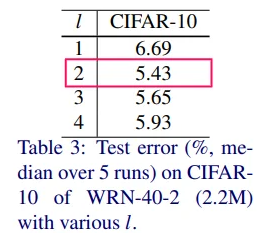
\includegraphics[width=6cm]{./capture/WideResNet.png}
  \caption{WideResNet内のResidual Blockの層の数に対するエラー率の遷移: Residual Block内では、l=1では表現力が足りず、l>=3の時は残差接続が減少して最適化が難しくなるため、l=2が最適という研究結果になっている。}
\end{figure}
WideResNetの表記「WRN-n-k」は、n層の畳み込みを持ち、幅(チャネル数)を$k$倍することを意味する。パラメータ数と計算量は$k$の二乗になる。$k=1$のときは元のResNetと同一で、$k>1$の時にWideResNetとなる。
ResNet-1001(パラメータ数:$10.2\times 10^6$)よりもWRN-40-4(パラメータ数:$8.9\times 10^6$)の方がパラメータ数が大幅に削減され、8倍高速になった。


\subsection{ファインチューニング}
ファインチューニングとは、転移学習の一種であり、事前学習モデルを用意し、バッチ正規化部分のパラメータだけを固定して、追加したタスクに加えて、事前学習モデル内も含めて、すべてのパラメータを再学習させる手法である。Tensorflow HubのResNetは、trainableをTrueに変更するだけで、ファインチューニングを行い、事前学習モデルの特徴を引き継ぎつつ、新しいタスクに適応した高精度モデルを簡単に作成することができる。

\clearpage
\section{EfficientNet}
\subsection{概要}
AlexNet以降は、CNNモデルを大規模にスケールアップすることで精度を改善するアプローチがトレンドだった (ResNet-18からResNet-200まである)。
スケールアップの変数は、幅(1層あたりのノード数)、深さ(層数)、解像度(入力画像の解像度)の3つである。
\begin{enumerate}
  \item 深さ($d$) : 表現力が高くなり、複雑な特徴表現を獲得できるようになる。
  \item 幅($w$) : 細かい特徴表現を獲得し、学習を高速化できるようになる。
  \item 解像度($r$) : 画像の特徴をより詳細に捉えることができるようになる。
\end{enumerate}
これらの変数のスケールアップにより、精度の向上が期待できたが、ある程度まで増やすと精度の向上は横ばいとなってしまう上に、演算量(FLOPS)は、$d\cdot w^2 \cdot r^2$で増加するため、モデルのサイズが大きくなると、計算リソースが不足する問題があった。
\par
2019年にGoogleが提案したEfficientNetは、効率的なスケールアップの規則を採用することで、計算量を抑えつつ、精度を向上させることに成功したモデルである。
\par
その規則とは、Compound Coefficent(複合係数)と呼ばれる1つの係数$\phi$で説明され、その係数を用いて一様にスケーリング可能になる。EfficientNetでは$d, w, r$が以下で定義される。
\begin{align}
  \text{depth} &: d = \alpha^{\phi} \\
  \text{width} &: w = \beta^{\phi} \\
  \text{resolution} &: r = \gamma^{\phi}\\
  \label{eq:EfficientNet4}
  \text{s.t. }  & \alpha \cdot \beta^2 \cdot \gamma^2 \approx 2 \\
  & \alpha \geq 1, \beta \geq 1, \gamma \geq 1
\end{align}
$\alpha, \beta, \gamma$はハイパーパラメータであり、それぞれは、\eqref{eq:EfficientNet4}の制約条件を満たすようにグリッドサーチで設定されるため、FLOPSは$\sim (\alpha \cdot \beta^2 \cdot \gamma^2)^{\phi} \approx 2^{\phi}$ と表され、計算リソースに対するモデルのスケールの見積もりがしやすくなる。例えば、$\phi=1$のときの最適値、$\alpha=1.2, \beta=1.1, \gamma=1.15$は、EfficientNet-B0と呼ばれるモデルであり、FLOPS$\sim 0.35$G、パラメータ数$\sim 5$Mである。
EfficientNet-B0のアーキテクチャは、図\ref{fig:EfficientNet}のように表されれ、EfficientNetは、EfficientNet-B0からEfficientNet-B7までの8つのモデルが提案されている。
\begin{figure}
  \centering
  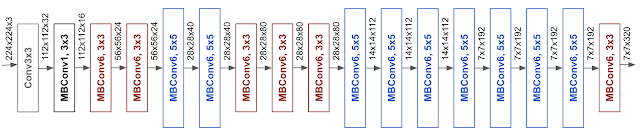
\includegraphics[width=15cm]{./capture/EfficientNet.png}
  \caption{EfficientNetの構造}
  \label{fig:EfficientNet}
\end{figure}


\subsection{Compound Scaling Method}
EfficientNetのCompound Scaling Methodは、モデルのスケールアップを効率的に行うための方法であり、以下の数式で表される
\begin{align}
  \label{eq:compound_scaling_1}
  \max_{\alpha, \beta, \gamma} & \text{Accuracy}(\mathcal{N}(d, w, r)) \\
  \label{eq:compound_scaling_2}
  \text{s.t. } &\mathcal{N}(d, w, r) = \bigodot_{i=1\cdots s} \hat{\mathcal{F}}_{i}^{d\cdot \hat{L}_i} (X_{\langle r\cdot \hat{H_i}, r\cdot \hat{W_i}, w\cdot \hat{C_i} \rangle })\\
  \label{eq:compound_scaling_3}
  &\text{Memory}(\mathcal{N}(d, w, r)) \leq \text{target memory}\\
  \label{eq:compound_scaling_4}
  &\text{FLOPS}(\mathcal{N}(d, w, r)) \leq \text{target FLOPS}
\end{align}
ここで、$\mathcal{N}(d, w, r)$は、深さ$d$, 幅$d$, 解像度$r$のネットワークを表し、$\hat{\mathcal{F}}^{L_i}(X_{\langle \hat{H_i}, \hat{W_i}, \hat{C_i} \rangle })$は$L_i$回繰り返す畳み込み層を表し、入力時の高さ$\hat{H_i}$、幅$\hat{W_i}$、チャンネル数$\hat{C_i}$を引数で取る。
\par
まず、式\eqref{eq:compound_scaling_1}は、モデルの精度を最大化するための目的関数である。
\par
式\eqref{eq:compound_scaling_2}は、モデルのアーキテクチャを表す関数を表し、$\odot_{i=1\cdots s}$は、モデル$\mathcal{N}$がs個のブロックから構成されていることを示す。Fは畳み込み層を表し、Lはブロックの中で何度Fを繰り返すかを表す。
\par
式\eqref{eq:compound_scaling_3}と、式\eqref{eq:compound_scaling_4}は、モデルのメモリとFLOPSが目標値以下であることを示す制約条件である。
\par
これらの式を解くことで、最適な$\alpha, \beta, \gamma$を求めることができる。

\clearpage
\section{Vision Transformer(ViT)}
\subsection{概要}
Vision Transformer(ViT)は、2020年にGoogleが提案した、画像認識のためのTransformerベースのモデルである。ViTは、画像をパッチと呼ばれる小さな領域に分割し、それぞれのパッチを系列(Sequence)データとしてTransformerに入力することで、画像認識を行う。ViTは、CNNベースのモデルと比較して、計算効率が高く、畳み込み層を用いないため、モデルの拡張が容易であるという特徴がある。ViTのアーキテクチャを図\ref{fig:ViT}に示す。
\begin{figure}[htbp]
  \centering
  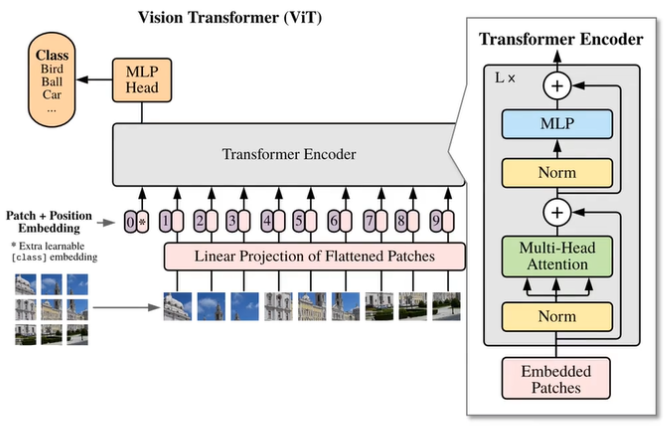
\includegraphics[width=10cm]{./capture/ViT.png}
  \caption{Vision Transformerのアーキテクチャ}
  \label{fig:ViT}
\end{figure}

ViTの処理は、以下の手順で行われる。
\begin{enumerate}
  \item 画像をパッチに分割する
  \item パッチ事にFlatten処理を行い、トークン系列を得る。
  \item Embedding表現(埋め込み表現)に変換する。
  \item CLS トークンを系列データの最初に負荷する。
  \item Positional Encodingを付加する。
  \item Transformerに入力する。
  \item 出力を取り出し、分類を行う。
\end{enumerate}
ここで、Flatten処理は、画像のパッチを1次元のベクトルに変換する処理である。また、Embedding表現は、トークンをベクトル表現に変換する処理であり、Inductive biasとHybrid Architectureという2つの表現方法がある。CLS トークンは、系列データの最初に配置され、系列データ全体の特徴を表すトークンである。
\par
ViTの計算過程は、数式を用いて以下のように表される。
\begin{align}
  \text{Input} & : x \in \mathbb{R}^{H \times W \times C}\\
  \text{Patch Embedding} & : \mathbb{X}_p \in \mathbb{R}^{N \times (C \times P^2)}\\
  & \left( \text{s.t. }  N = \frac{H \times W}{P^2} \right) \\ 
  \text{Class Token} & : \mathbb{X}_{cls} \in \mathbb{R}^{1 \times (C \times P^2)}\\
  \text{Encoder Input} & : \mathbb{Z}_0 = \left[ X_{\text{cls}}; X_p^1 \mathbb{E}; X_p^2 \mathbb{E}; \cdots ;X_p^N \mathbb{E} \right] + \mathbb{E}_{pos}\\
  & \left( \text{s.t. }  \mathbb{E} \in \mathbb{R}^{(C \times P^2) \times D}, \mathbb{E}_{pos} \in \mathbb{R}^{(N+1) \times D} \right)\\
  \text{Transformer(l layer)} &: \mathbb{Z'}_l = \text{MSA}( \text{LN}(\mathbb{Z}_{l-1}) ) + \mathbb{Z}_{l-1}\\ 
  \text{Transformer(Output)} & : \mathbb{Z}_l = \text{MLP}(\text{LN}(\mathbb{Z'}_l)) + \mathbb{Z'}_l\\
  \text{Encoder Output} & : \mathbb{Y} = \text{LN}(\mathbb{Z}_l^0) 
\end{align}
MSAは、Multi-Head Self-Attentionを表し、MLPは、Multi-Layer Perceptronを表す。また、LNは、Layer Normを表す。
Encoder OutputはD次元の特徴量出力、MLP Headに入力され、最終的な出力が得られる。MLP HeadではD次元をKクラスに変換する。ファインチューニング時には、MLP Headのみを学習させることで、新しいタスクに適応したモデルを作成することができる。また、Position Embedingを変更することで、事前学習よりも高解像度の画像に対応したモデルを作成することができる。
\par
ViTは、計算量が増えるほど精度が向上するという特徴がある。また、ViTは、CNNベースのモデルと比較して、計算効率が高く、畳み込み層を用いないため、モデルの拡張が容易であるという特徴がある。

\paragraph{参考文献}
\begin{enumerate}
  \item スキップ接続 (Skip connection)  CVMLエキスパートガイド \url{https://cvml-expertguide.net/terms/dl/inter-layer-connection/skip-connection/}
  \item 【初心者にも分かりやすく】画像認識モデルのResNetの要点を解説 \url{https://dx-consultant-fast-evolving.com/resnet/}
  \item 【E資格まとめ】ResNetとWideResNet \url{https://tt-tsukumochi.com/archives/8991}
  \item  ResNetの改良モデルWideResNetを詳細解説! \url{https://deepsquare.jp/2021/08/wideresnet/}
  \item EfficientNet: Rethinking Model Scaling for Convolutional Neural Networks , Tan and Le 2019 \url{https://arxiv.org/abs/1905.11946}
  \item EfficientNet: Improving Accuracy and Efficiency through AutoML and Model Scaling  \url{https://research.google/blog/efficientnet-improving-accuracy-and-efficiency-through-automl-and-model-scaling/}
\end{enumerate}

\clearpage
\section{実装演習キャプチャ}
%------------
%ResNet
%------------
\subsection{ResNet}
\begin{figure}[htbp]
  \centering
  \includegraphics[width=10cm]{C:/Users/hiroh/Videos/Captures/4_1_transfer-learning/Arc 2024_07_04 22_00_53.png}
\end{figure}
\begin{figure}[htbp]
  \centering
  \includegraphics[width=10cm]{C:/Users/hiroh/Videos/Captures/4_1_transfer-learning/Arc 2024_07_04 22_01_00.png}
\end{figure}
\begin{figure}[htbp]
  \centering
  \includegraphics[width=10cm]{C:/Users/hiroh/Videos/Captures/4_1_transfer-learning/Arc 2024_07_04 22_01_35.png}
\end{figure}
\begin{figure}[htbp]
  \centering
  \includegraphics[width=10cm]{C:/Users/hiroh/Videos/Captures/4_1_transfer-learning/Arc 2024_07_04 22_01_47.png}
\end{figure}
\begin{figure}[htbp]
  \centering
  \includegraphics[width=10cm]{C:/Users/hiroh/Videos/Captures/4_1_transfer-learning/Arc 2024_07_04 22_01_52.png}
\end{figure}
\begin{figure}[htbp]
  \centering
  \includegraphics[width=10cm]{C:/Users/hiroh/Videos/Captures/4_1_transfer-learning/Arc 2024_07_04 22_01_57.png}
\end{figure}
\begin{figure}[htbp]
  \centering
  \includegraphics[width=10cm]{C:/Users/hiroh/Videos/Captures/4_1_transfer-learning/Arc 2024_07_04 22_02_00.png}
\end{figure}
\begin{figure}[htbp]
  \centering
  \includegraphics[width=10cm]{C:/Users/hiroh/Videos/Captures/4_1_transfer-learning/Arc 2024_07_04 22_02_04.png}
\end{figure}

\clearpage
%------------
%WideResNet
%------------
\subsection{WideResNet}
\begin{figure}[htbp]
  \centering
  \includegraphics[width=10cm]{C:/Users/hiroh/Videos/Captures/4_2_wide_resnet/Arc 2024_07_04 22_45_05.png}
\end{figure}
\begin{figure}[htbp]
  \centering
  \includegraphics[width=10cm]{C:/Users/hiroh/Videos/Captures/4_2_wide_resnet/Arc 2024_07_04 22_45_12.png}
\end{figure}
\begin{figure}[htbp]
  \centering
  \includegraphics[width=10cm]{C:/Users/hiroh/Videos/Captures/4_2_wide_resnet/Arc 2024_07_04 22_45_16.png}
\end{figure}
\begin{figure}[htbp]
  \centering
  \includegraphics[width=10cm]{C:/Users/hiroh/Videos/Captures/4_2_wide_resnet/Arc 2024_07_04 22_45_21.png}
\end{figure}
\begin{figure}[htbp]
  \centering
  \includegraphics[width=10cm]{C:/Users/hiroh/Videos/Captures/4_2_wide_resnet/Arc 2024_07_04 22_45_26.png}
\end{figure}
\begin{figure}[htbp]
  \centering
  \includegraphics[width=10cm]{C:/Users/hiroh/Videos/Captures/4_2_wide_resnet/Arc 2024_07_04 22_45_30.png}
\end{figure}
\begin{figure}[htbp]
  \centering
  \includegraphics[width=10cm]{C:/Users/hiroh/Videos/Captures/4_2_wide_resnet/Arc 2024_07_04 22_45_37.png}
\end{figure}

\end{document}